\documentclass{article}

\usepackage{mhchem} % Package for chemical equation typesetting
\usepackage{siunitx} % Provides the \SI{}{} command for typesetting SI units
\usepackage{pdfsync}
\usepackage[english]{babel}
\usepackage{fullpage}
\usepackage{amsmath}
\usepackage[table]{xcolor}
\usepackage{multirow}
\usepackage{graphicx}
\usepackage{circuitikz}
\usepackage{caption}
\usepackage{subcaption}
\usepackage{float}
\usepackage{verbatim}
\usepackage{eso-pic}
\usepackage[toc,page]{appendix}
\usepackage[linkbordercolor={white}]{hyperref}
\usepackage{nameref}
\usepackage{listings}
\usepackage{mcode}
\usepackage{graphicx} % Required for the inclusion of images

\setlength\parindent{0pt} % Removes all indentation from paragraphs

%\usepackage{times} % Uncomment to use the Times New Roman font

%----------------------------------------------------------------------------------------
%	DOCUMENT INFORMATION
%----------------------------------------------------------------------------------------

\title{Report System Validation Project \\ Modeling a Bridge's Control System\\ Creating a safety layer with mCRL2 using Labelled Transition Systems} % Title

\author{Aimee \textsc{Ferouge} 4014030 \\Wieger \textsc{IJntema} 4034570 \\Arian \textsc{Stolwijk} 4001079} % Author name

\date{\today} % Date for the report

\begin{document}

\maketitle % Insert the title, author and date

\begin{center}
\begin{tabular}{l r}
Date Performed: & Januari, 2013 \\ % Date the experiment was performed
Instructor: & J. J. A. Keiren % Instructor/supervisor
\end{tabular}
\end{center}

% \begin{abstract}

 %\end{abstract}

%----------------------------------------------------------------------------------------
%	Introduction
%----------------------------------------------------------------------------------------


\section{First deliverable}
\subsection{Introduction}

As has been pointed out by the incident at the Ketelbrug between Emmeloord and Lelystad, bridges require a very precise control system.  Many examples exist where bridges are not opened or closed properly, where bridge components break down or the bridge is being stuck in a particular state. The goal of this project is to design a satefy layer that can be added to the main control interface, in order to capture all possible situations and failures.
Throughout the report, we make use of the following assumptions:
%
\begin{itemize}
	\item If three or four sensors detect an open/closed bridge, the bridge can be considered open/closed
	\item If only the four sensor have a 50/50 detection on the bridge deck, the bridge should remain in its current position (open/closed)
	\item A barrier can only be considered to be down when the majority of the sensors detect a lowered barrier
\end{itemize}
%
In this section, the desired behaviour of the bridge is being determinated and defined. Section \ref{sec:glob} contains the global requirements that will be met in our system. Specific interactions that can be performed by the bridge are discussed in Section \ref{sec:act}, whereas Section \ref{sec:trans} translates these interactions into the requirements stated earlier.
%----------------------------------------------------------------------------------------
%	De rest
%----------------------------------------------------------------------------------------
\subsection{Global Requirements}
\label{sec:glob}

Using the Project Guide\footnote{J. J. A. Keiren, System Validation (IN4387) Project Guide, VU University Amterdam, november 2013} as a source for the desired behaviour, the following requirements are defined:
\\
\\
\textbf{Opening the bridge}
	\begin{enumerate}
  	\item Switching on pre signs should be the first action when opening the bridge
		\item Stop signs cannot be lit as long as the pre lights have not been lit
		\item Barriers cannot be lowered if the stop signs have not been lit
		\item Bridge can only be unlocked when all barriers are down
		\item The deck can only lifted when both locks are unlocked
   \newcounter{enumTemp}
   \setcounter{enumTemp}{\theenumi}
 \end{enumerate}
  
\textbf{Closing the bridge}
  \begin{enumerate}
    \setcounter{enumi}{\theenumTemp}
  	\item Bridge can only be locked when the deck is down
		\item Barriers can only be up when the bridge is locked by at least 
		\setcounter{enumTemp}{\theenumi}
  \end{enumerate}
 
\textbf{Functional requirements}
	\begin{enumerate}
	
			\item The bridge should be able to be opened when a ship approaches
			\item The bridge should be able to close in order to let cars pass
			\item The first barrier to be encountered by the cars is lowered earlier than the second in order to enable cars to leave the bridge
		\setcounter{enumTemp}{\theenumi}
	\end{enumerate}

\textbf{Failure}
	\begin{enumerate}
		\setcounter{enumi}{\theenumTemp}
			\item The stop signs can only be lit if at least one pre signs is being lit at each side of the bridge
			\item The barriers can only be lowered if both stop signs are being lit at each side of the bridge
			\item If the motor is in the 'broken' status, the bridge may not be opened
		\setcounter{enumTemp}{\theenumi}
	\end{enumerate}

\subsection{Interactions}
\label{sec:act}

\begin{table}[htb]%
\begin{tabular}{lll}
      \textbf{Interaction} &	\textbf{Descripton}	&	\textbf{Parameters}\\
      \hline
      \mcode{open} & Opens the bridge &\\
      \mcode{close} & Closes the bridge &\\
      \mcode{getSign} & Checks te status of a specific sign & Sign\\
      \mcode{setSign} & Switches a sign on or off & Sign, status \\
      \mcode{getBarrier} & Checks the status of a specific barrier & Barrier\\
      \mcode{setBarrier} & Lowers of lifts a specific barrier & Barrier, status\\
      \mcode{getLock} & Checks the status of a specific locking pin & Lock\\
      \mcode{setLock} & Locks or unlocks a specific locking pin & Lock, status\\
      \mcode{getDeck} & Checks the status of the bridge deck &\\
      \mcode{setDeck} & Lowers or liftst the bridge deck & Status\\
      \mcode{motorStatus} & Checks the status of the motor\\
\end{tabular}
\caption{All interactions to be performed by the safety layer of the control system.}
\label{tab:act}
\end{table}

\subsection{Architecture}
\label{sec:trans}

Three parallel processes exist being \emph{signs}, \emph{barriers} and \emph{bridge}. \emph{Signs} handles the control of the lights, whereas \emph{barriers} handles the barriers and \emph{bridge} the locks and the deck.

\emph{Signs} is the first one to be executed when an \mcode{open} or \mcode{close} command is given. After first lighting the pre signs and then the stop signs, control is given to the \emph{barriers} process.

\emph{Barriers} makes sure all barriers are lowered if the stop signs are lit. When this is the case, \emph{bridge} takes over.

\emph{Bridge} handles the lifting and lowering of the bridge deck. Only when all barriers are down, the two locks of the bridge are removed and the deck can be moved up and down. When finishing this movement, control is given back first to \emph{barriers} and finally back to \emph{barriers}.

Figure \ref{fig:arch} shows a sequence diagram of how the control shifts between these parallel processes.
%
\begin{figure}%
\centering
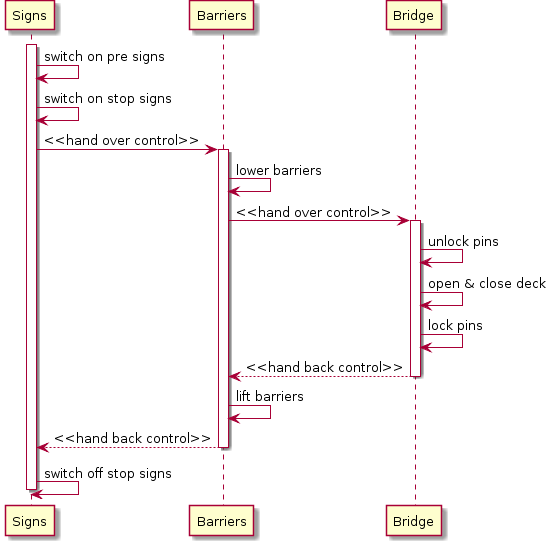
\includegraphics[width=0.5\columnwidth]{Architecture}%
\caption{Sequence diagram of control flow between parallel processes \emph{signs}, \emph{barriers} and \emph{bridge}.}%
\label{fig:arch}%
\end{figure}

\subsection{Translation of Requirements in Terms of Interactions}

In order to create a model for the bridge in mCRL2, which is modeling software used for system validation, the requirements have to expressed in terms of the previous stated interactions. At the moment, we are still rewriting these translations after the feedback we received during last week's meeting. The following translations are from last week.

\begin{enumerate}
	\item \textbf{Stop signs cannot be lit as long as the pre lights have not been lit}
	When setSign is set on for all stop-signs, then check for all pre-signs if getSign is on before, and not off intermediate.
	Else when setSign is set on for all stop-signs, then check for three pre-signs if getSign is on before, and not off intermediate.
	Else, give error and stop.

	\item \textbf{Barriers cannot be closed if the stop signs have not been lit}
	When setBarrier is set down for all barriers, then check for all stop-signs if getSign is on before, and not off intermediate.
	Else when setBarrier is set down for all barriers, then check for three stop-signs if getSign is on before, and not off intermediate.
	Else, give error and stop.

	\item \textbf{Bridge can only be unlocked when all barriers are down}
	When setLock is set unlocked for all locks, then check for all barriers if getBarrier is down before, and not up intermediate.
	Else, give error and stop.

	\item	\textbf{The deck can only lifted when it is completely unlocked}
	When setDeck is set up for the bridge deck, then check for all locks if getLock is unlocked before, and not locked intermediate.
	Else, give error and stop.

	\item \textbf{Bridge can only be locked when the deck is down}
	Always when setLock(L2), then getDeck is down before, and not changed intermediately.
	Always when setLock(L1), then getDeck is down before, and not changed intermediately.

	\item \textbf{Barriers can only be up when the bridge is locked by at least one lock}
	Always when setBarrier(B, up), getLock(L1) or getLock(L2) are enabled, and not disabled intermediately.

	\item \textbf{Stop sign can be shut off only when the barriers are up}
	Always when setSign(S, off), for each B1, B2, B3, B4, getBarier should be up before, and not changed intermediately.

	\item \textbf{The bridge should be able to be opened when a ship approaches}
	When giving the open command, somewhere in the process setDeck should be set to up.

	\item \textbf{The bridge should be able to close in order to let cars pass}
	When giving the close command, somewhere in the process setDeck should be set to down.

	\item \textbf{The first barrier to be encountered by the cars is lowered earlier than the second in order to enable cars to leave the bridge}
	Always when setBarrier(B2, down), getBarrier(B1) must be down or else the process is stopped. 
	Always when setBarrier(B3, down), getBarrier(B4) must be down or else the process is stopped. 

	\item \textbf{The stop signs can only be lit if at least one pre signs is being lit at each side of the bridge}
	Always when setSign(S1, on) or setSign(S2, on), at least one status of getSign(P1) or getSign(P2) must be on. If not, the process is stopped.
	Always when setSign(S1, on) or setSign(S2, on), at least one status of getSign(P1) or getSign(P2) must be on. If not, the process is stopped.

	\item \textbf{The barriers can only be lowered if both stop signs are being lit at each side of the bridge}
	Always when setBarrier(B1, down), getSign(S1) and getSign(S2) must be down. If not, the process is stopped.
	Always when setBarrier(B1, down), getSign(S1) and getSign(S2) must be down. If not, the process is stopped.

	\item \textbf{If the motor is in the 'broken' status, the bridge should stay in the current position}
	Whenever motorStatus has been changed to broken and has not changed back to stopped, moving up or moving down, no components may be set anymore.

\end{enumerate}

\section{Second Deliverable}

The full report, draft version.



%----------------------------------------------------------------------------------------
%	BIBLIOGRAPHY
%----------------------------------------------------------------------------------------
%
%\bibliographystyle{unsrt}
%
%\bibliography{sample}
%
%----------------------------------------------------------------------------------------


\end{document}


